\begin{homeworkProblem}

    在网上寻找任意类型的、与信息检索有关的任意可运行系统(针对text、image、video、audio等均可。商用系统及尚处于研究中的demo系统都可以。
    我们鼓励大家尝试花样尽可能多的“搜索引擎”,查询query可以不限于文字,例如可以是一张图片),键入一定量的、能够说明问题的相关query,测试其功能,对结果给出某种形式的定量评估,并根据自己的理解作相应分析。
    \\

    \textbf{\large Report}

    使用 Google Search 搜索 “优胜美地” 相关信息。
    \\

    \textbf{Part One}

    使用 \href{https://www.google.com}{Google 文本搜索},输入关键词“优胜美地”。首页条目如下:
    
    \begin{enumerate}
        \item 优胜美地『玩哪儿网』 | 美西旅行团全线7折起 | wannar.com‎
        \item Yosemite National Park (U.S. National Park Service)
        \item 優勝美地國家公園- 维基百科,自由的百科全书
        \item Yosemite National Park | Lodging \& Year Round Activities ...
        \item Yosemite National Park | Lodging, Camping, Attractions
        \item 优胜美地国家公园景点 - 目的地 - 穷游
        \item 优胜美地国家公园Yosemite national park - 目的地 - 穷游
        \item 优胜美地国家公园 - 马蜂窝
        \item 优胜美地国家公园 - 携程攻略
        \item Images for 优胜美地
        \item 聚焦:优胜美地国家公园| Visit California
    \end{enumerate}

    在首页显示的 11 个条目中,第1条显示为“Ad”为广告条目。其余10条中:

    \begin{enumerate}
        \item 第2、4、5、11条为优胜美地官方中英文景点介绍页面
        \item 第3条为维基百科页面
        \item 第6、7、8、9条为国内主流的旅游网站
        \item 第10条为图片搜索
    \end{enumerate}

    以上结果表明该任务的文本搜索基本能满足了解一个地点、准备旅游攻略这两个用户要求。
    \\

    \pagebreak

    \textbf{Part Two}

    使用 \href{https://images.google.com}{Google 图片搜索},给定图片如下:

    \begin{figure}[!h]
        \centering
        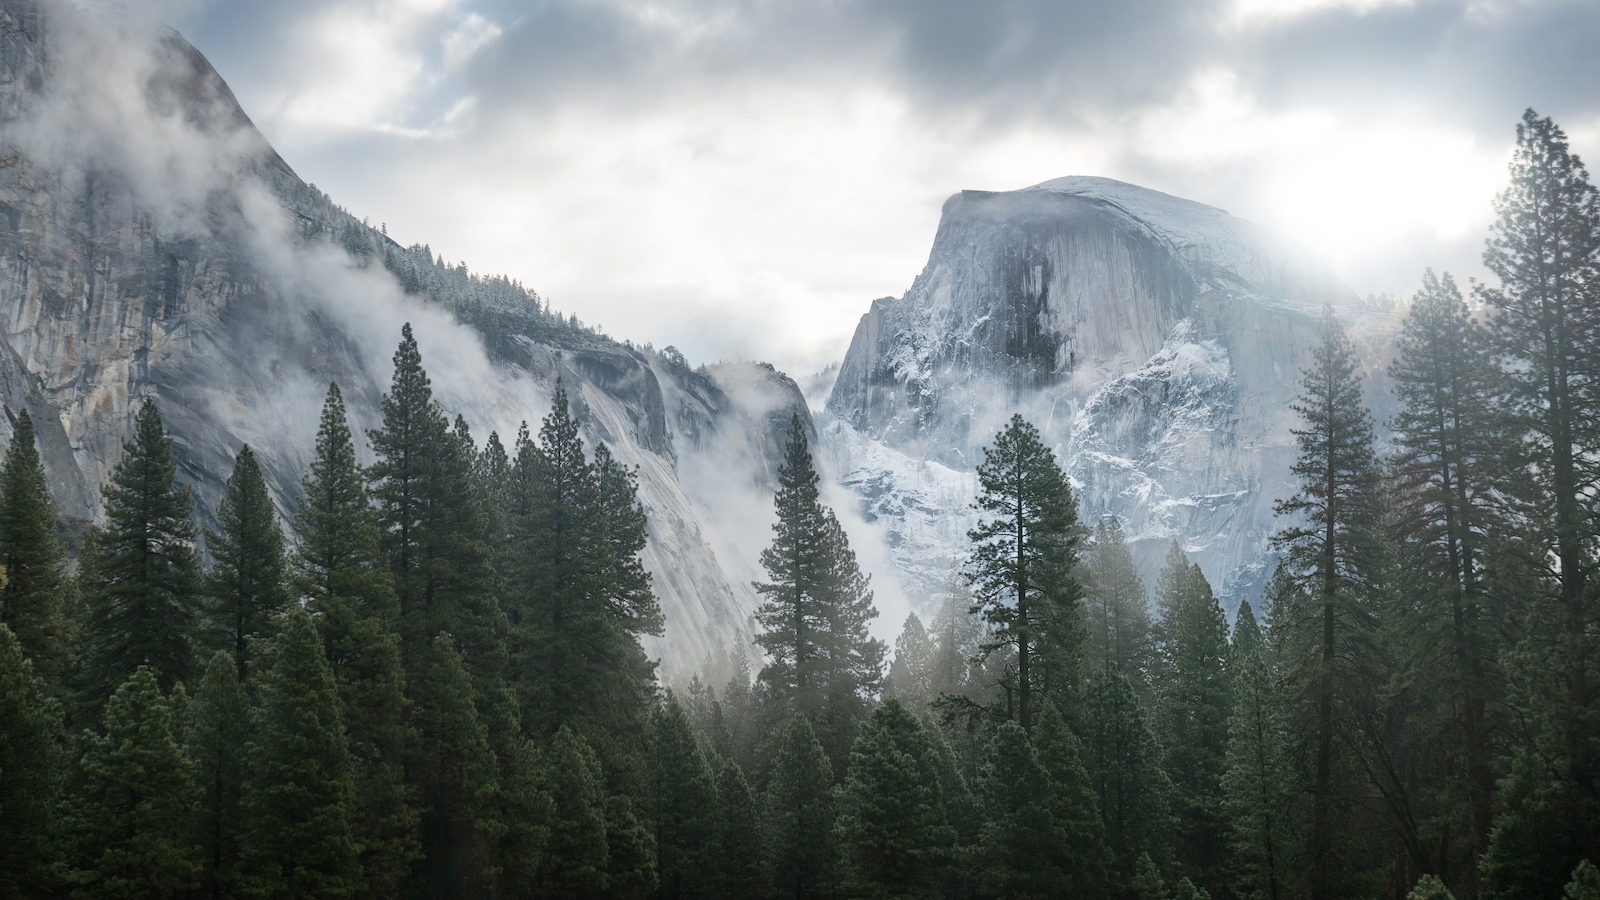
\includegraphics[width=0.8\textwidth]{images/yosemite.jpg}
        \caption{优胜美地图片(同时是 macOS 10.10 的壁纸)}
    \end{figure}

    结果如下:

    \begin{enumerate}
        \item Refurbished 12-inch MacBook 1.1GHz Dual-core Intel Core M - Silver ...
        \item Amazon.com : Apple Macbook 12" Laptop w/ Retina Display - (256GB ...
        \item Here are all of OS X Yosemite's beautiful new wallpapers | 9to5Mac
        \item 20 Beautiful Apple macOS 5K Wallpapers And HD Backgrounds
        \item Passport Summer Camp - Tampa Metropolitan Area YMCA
        \item Yosemite, 5k wallpapers, forest, OSX, apple, mountains | km's nice ...
        \item Free wallpaper | Wallpaper | Pinterest | Wallpaper, Mac os wallpaper ...
    \end{enumerate}

    由于该图片是 macOS 10.10 的壁纸,发现搜索结果均为 mac, apple, wallpaper 等关键词,没有与优胜美地景点相关的项。

    \pagebreak

    \begin{figure}[!h]
        \centering
        \includegraphics[width=0.8\textwidth]{images/DSC00129.jpg}
        \caption{优胜美地实拍照片}
    \end{figure}

    结果如下:

    \begin{enumerate}
        \item Glacier Point - Yosemite National Park (U.S. National Park Service)
        \item Glacier Point Yosemite | Discover Yosemite Glacier Point
        \item Visually similar images
    \end{enumerate}

    与上一个输入不同,此照片为优胜美地的实拍照片,可以看到总共仅有3个结果,均为优胜美地官网的介绍,表明该景点名为 Glacier Point,包含进一步的介绍。在第三项 Visually similar images 中可以看到类似的关于该处的图片。

\end{homeworkProblem}

\pagebreak
